\capitulo{4}{Metodología}
En este capítulo voy a desarrollar los datos, las técnicas y métodos utilizados durante el proyecto. 
\section{Descripción de los Datos}
Para la realización del proyecto, no se han utilizado datos predefinidos por bases de datos, APIs públicas u otras fuentes de información.Los datos que aparecen son los obtenidos por los sensores durante las pruebas del dispositivo.
\section{Técnicas metodológicas de programación}
En esta sección se detallan las técnicas metodológicas de programación empleadas en el desarrollo del proyecto. 
\subsection{Lenguajes de programación}
En el proyecto empleé los siguientes lenguajes de programación especialmente seleccionados para cumplir con los requisitos de este.
\subsubsection{\textit{C++}}
Lenguaje de programación compilado y multiparadigma, caracterizado por su enfoque imperativo y orientado a objetos. Además, incluye el uso de programación general y funcional.
Muy utilizado en la creación de programas para la creación de interfaces y videojuegos.\cite{C++}\footnote{Pagina web con información de C++\cite{C++}.}

Se ha utilizado este lenguaje para la implementación de toda la lógica asociada a la placa Elegoo.
\subsubsection{\textit{Python}}
Python es un lenguaje alto de programación altamente usado, interpretado y multiplataforma. Diseñado para ser fácil de leer y escribir.
Ampliamente utilizado en el desarrollo web, ciberseguridad, aprendizaje automático, desarrollo de aplicaciones o la automatización de tareas, entre muchas otras aplicaciones.\cite{Python}\footnote{Pagina web con información de Python\cite{Python}.}
\subsubsection{\textit{Bash}}
Bash es un lenguaje de comandos y shell de Unix/Linux, también conocido como shell scripting o comandos de terminal.
Se ejecuta en una terminal o ventana de texto.\cite{Bash}\footnote{Pagina web con información de Bash\cite{Bash}.}

En este proyecto ha sido utilizado en la terminal de Rstudio para la creación de archivos, actualización de GitHub entre otras tareas.
----
\subsection{Bibliotecas}
La bibliotecas o librerías son un conjunto de funciones, clases y recursos ya escritos que se pueden utilizar de manera libre para agilizar procesos. 

\subsubsection{json}
Librería que permite la edición y adicción de documentos JSON.
\subsubsection{os}
Librería que permite la interacción con el sistema operativo.
\subsubsection{pandas}
Librería que permite el análisis y manipulación de datos.
\subsubsection{openpyxl}
Librería que permite leer, modificar y escribir archivos excel.
\subsubsection{Kivy}
Librería que permite la creación de interfaces gráficas de usuario(GUI).\cite{kivy}\footnote{Pagina web con información de kivy y documentación\cite{kivy}.}
\section{Entornos y aplicaciones}
En esta sección voy a realizar una recopilación de aplicaciones y entornos que he utilizado para la realización del proyecto, todas ellas explicadas y utilizadas en diferentes asignaturas del grado.
\subsection{Overleaf}
Herramienta en línea que permite redactar,editar,exportar y compartir con otros usuarios documentos científicos en formato LaTeX.

En este proyecto, se utiliza Overleaf para la creación de este documento y el anexo.
\subsection{RStudio}
RStudio es un entorno de software libre para computación estadística y gráficos. Tiene la capacidad de ejecutarse y compilarse en una amplia variedad de plataformas como Linux,MAC y Windows.\cite{Rstudio}\footnote{Pagina web con información de Rstudio\cite{Rstudio}.}

En este proyecto, se utiliza RStudio para realizar una unión entre el repositorio de GitHub y la carpeta de mi escritorio del ordenador donde voy avanzando el proyecto.
\subsection{GitHub}
GitHub es una plataforma basada en la nube cuya finalidad es almacenar,compartir y trabajar en conjunto con otros usuarios. 
Además, permite tener un seguimiento del trabajo, lo que permite ver todas las versiones que se van realizando de este mismo.\cite{GitHub}\footnote{Pagina web de GitHub\cite{GitHub}.} 

En este proyecto, GitHub se ha utilizado para realizar un seguimiento del proyecto, permitiendo que tanto el tutor como los miembros del tribunal puedan visualizar los cambios realizados y participar activamente en el proceso.
\subsection{Tinkercad}
Tinkercad es una aplicación web que permite la realización de diseños en 3D, la realización de circuitos y la posibilidad de escribir programas para dar vida a los diseños mediante la codificación.

En este proyecto, ha sido utilizada para la realización de la simulación del diseño del circuito electrónico, ya que permite utilizar diseños electrónicos ya hechos, modificarlos, añadir más componentes o empezar desde 0 un circuito.
\subsection{Visual Studio Code}
Visual Studio Code es una aplicación que funciona como editor de código fuente, personalizable y multiplataforma.
Permite al usuario la creación y edición de archivos en múltiples lenguajes y formatos, desde texto plano hasta YAML, pasando por JSON, Markdown, XML y muchos otros; además, gracias a sus múltiples extensiones, permite, entre otras cosas, el control de versiones con la extensión de GitHub o incluso el uso de IA con la extensión de Copilot.

En este proyecto, ha sido utilizada para realizar la interfaz y establecer la comunicación con la placa Elegoo, la elección de este editor se debió a las características mencionadas anteriormente, la facilidad de uso y la versatilidad, permitiendo un desarrollo ágil y eficiente del proyecto.
\subsection{Freecad}
Freecad es una aplicación multiplataforma, de código abierto y completamente gratuita, que permite al usuario crear diseños en tres dimensiones.
Es un modelador 3D paramétrico de código abierto, permitiendo así diseños lo mas proximos a la realidad.

En este proyecto, ha sido utilizada para realizar un modelo 3D para el proyecto.\cite{freecad}\footnote{Pagina web con información y posibilidad de descarga de freecad\cite{freecad}.} 

\section{Herramientas}
En esta sección voy a exponer y explicar las herramientas que he utilizado en el proyecto.
\subsection{Placa de Elegoo uno R3}
Placa de Arduino es una placa de desarrollo de código abierto. 
Integra el microcontrolador chip Atmel ATMEGA+328P principal y un ATmega16U2 para la comunicación con USB. \cite{Elegoo}\footnote{Pagina web con información de placa Elegoo\cite{Elegoo}.}

Esta formado con 14 pines digitales, 6 pines analógicos, 5 pines de energía, un puerto de USB para la conexión con el ordenador, un conector para la alimentación, un botón de reinicio,un resonador de cerámica de 16 MHz, leds indicadores y los puertos I2C y SPI.\cite{Arduino}\footnote{Pagina web con información de Arduino\cite{Arduino}.}
En la \textit{Figura \ref{fig:Placa Elegoo}} se puede ver una imagen del componente.
\begin{figure}[h]
        \centering
        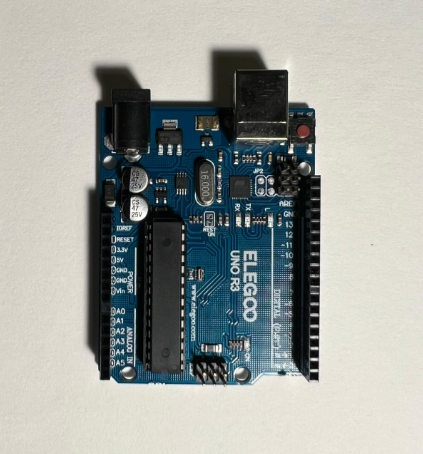
\includegraphics[angle=90,width=0.6\textwidth]{img/placa elegoo.png}
        \caption{Placa Elegoo}
        \label{fig:Placa Elegoo}
    \end{figure}

\subsection{Cables Dupont}
Alambres de metal conductor recubiertos de un plástico aislante flexibles que permiten las conexiones entre los propios componentes de la protoboard o entre la protoboard y la placa de Elegoo. En la \textit{Figura \ref{fig:cable_dupont}} se puede ver una imagen del componente.
\begin{figure}[h]
        \centering
        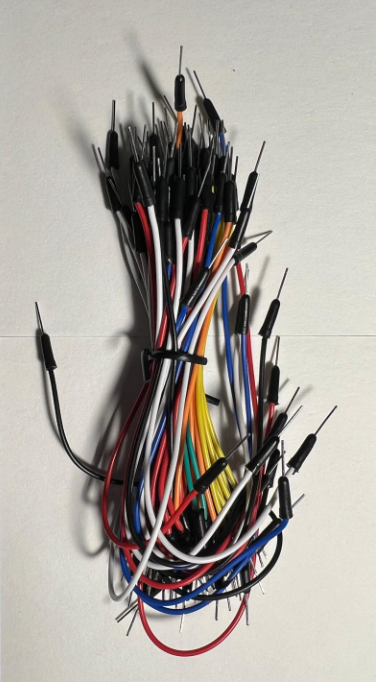
\includegraphics[angle=90,width=0.6\textwidth]{img/cable_dupont.png}
        \caption{Cables}
        \label{fig:cable_dupont}
    \end{figure}
   
\subsection{Cable USB}
Conector que une la placa Elegoo con el ordenador, permite introducir las instrucciones programadas en el ordenador en placa Elegoo. En la \textit{Figura \ref{fig:Cable USB}} se puede ver una imagen del componente.
\begin{figure}[h]
        \centering
        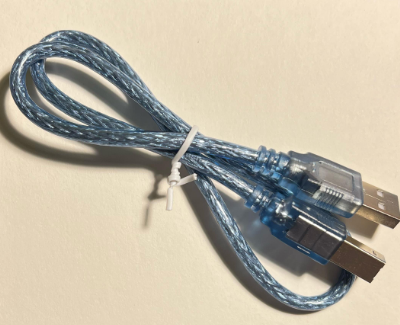
\includegraphics[width=0.5\textwidth]{img/cable usb.png}
        \caption{Cable USB}
        \label{fig:Cable USB}
    \end{figure}
   
\subsection{Resistencias}
Componentes electrónicos que limitan el flujo de la energía eléctrica en el circuito, son una medida de la oposición al flujo de corriente.  En la \textit{Figura \ref{fig:Resistencias}} se puede ver una imagen del componente.\cite{Resistencia}\footnote{Pagina web con información de las resistencias\cite{Resistencia}.}
\begin{figure}[h]
        \centering
        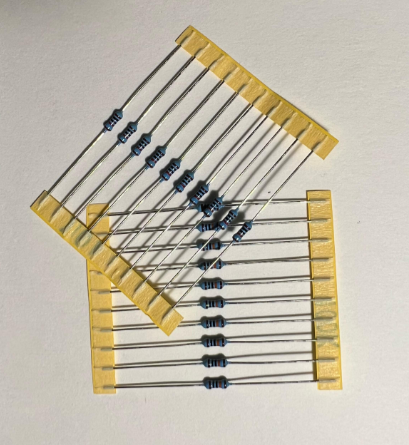
\includegraphics[width=0.5\textwidth]{img/Resistencias.png}
        \caption{Resistencia}
        \label{fig:Resistencias}
    \end{figure}
    
\subsection{Protoboard}
También llamada placa de pruebas, permite la creación de circuitos electrónicos.Es una matriz con orificios interconectados que permiten la inserción de componentes eléctricos. En la \textit{Figura \ref{fig:Protoboard} } se puede ver una imagen del componente.
\begin{figure}[h]
        \centering
        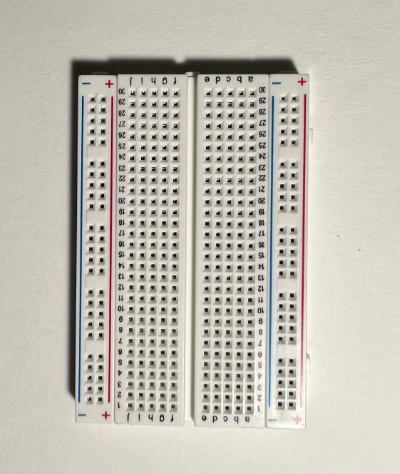
\includegraphics[angle=90,width=0.5\textwidth]{img/Protoboard.png}
        \caption{Protoboard}
        \label{fig:Protoboard}
    \end{figure}
\subsection{Posibles sensores}
En esta subsección se presentarán los sensores investigados para la realización del proyecto, el sensor seleccionado y el porqué de su selección.
\subsubsection{\textit{{Sensor fuerza resistivo}}}
Los sensores de fuerza resistivos son sensores capaces de detectar la presión o fuerza que se les ejerce.
Como su propio nombre dice, necesita para su uso una resistencia, la cual actúa como divisor de voltaje.
\subsubsection{\textit{{Células de carga}}}
Las células de carga son herramientas muy utilizadas en la industria para las mediciones de fuerza,compresión y tensión.
Son un tipo de transductores que convierten la fuerza aplicada  en una señal eléctrica medible. \cite{Celula_Carga}\footnote{Pagina web con información sobre las celulas de carga\cite{Celula_Carga}.}
Existen múltiples tipos de los cuales destacamos los siguientes:
    \begin{itemize}
        \item Células de cargas mecánicas: miden la fuerza mecánica al aplicarle un objeto, miden pesos.
        \item Células de carga extensométricas: miden deformaciones locales según su posición.La medida de la fuerza es determinada por la integración de los valores de cada valor individual, formado por un transductor de fuerza y un elemento elástico.\cite{celulas_extensométricas}\footnote{Pagina web con información de las células de carga de tipo extensométricas\cite{celulas_extensométricas}.}
        \item Células de carga hidráulicas:dispositivo llenó de un líquido con tiene una presión de precarga, al aplicar la fuerza aumenta la presión del líquido que es medida por un transductor de presión.
        \cite{Celulas_hidraulicas}\footnote{Pagina web con información de las células de carga de tipo hidraulicas\cite{Celulas_hidraulicas}.}
        \item Células de carga piezoélectricas: miden fuerzas dinámicas o cuasistáticas, tanto de tracción como compresión.Muy sensibles y rápidas.
        \cite{Celulas_piezoelectricas}\footnote{Pagina web con información de las células de carga de tipo piezoélectricas \cite{Celulas_piezoelectricas}.}
    \end{itemize}
En la \textit{tabla \ref{tab:comparacion_sensores}} se realiza un resumen donde se expondrán el tipo, características y precio aproximado de cada una de ellas.
\begin{table}[j]
\centering
\begin{tabular}{|l|p{8cm}|c|}
\rowcolor[HTML]{BFBFBF} 
\hline
\textbf{Tipo} & \textbf{Características de medición} & \textbf{Precio} \\
\hline
Células de carga mecánica & Rango de medición limitado, respuesta lenta, bajo costo, bajo mantenimiento & 10-200€ \\
\hline
Células de carga extensiométricas & Rango amplio (hasta 50 kN o más), buena precisión, alta estabilidad & 30-200€ \\
\hline
Células de carga hidráulicas & Medición de fuerzas grandes (hasta 100 kN), sin electrónica, resistente a ambientes hostiles & 50-300€ \\
\hline
Células de carga piezoeléctrica & Aproximadamente de 10 N a 300 kN, de precisión muy alta, ideal para fuerzas dinámicas & 60-500€ \\
\hline
Sensor de fuerza resistivo & Aproximadamente de 0-300N, precisión alta y de pequeño tamaño & 7-30€ \\
\hline
\end{tabular}
\caption{Tabla de comparación de sensores de fuerza}
\label{tab:comparacion_sensores}
\end{table}

Tras comparar los distintos sensores según su precio, características e integración, he concluido que los sensores de fuerza resistivos son la mejor opción para llevar a cabo el proyecto.

\subsection{{Sensor de fuerza resistivo}}
Como se ha explicado anteriormente los sensores de fuerza resistivos son sensores capaces de medir la fuerza ejercida con el uso de resistencias.

Para el proyecto se ha utilizado el sensor MD30-60 capaz de medir de 0 a 30Kg. 
\begin{figure}[h]
        \centering
        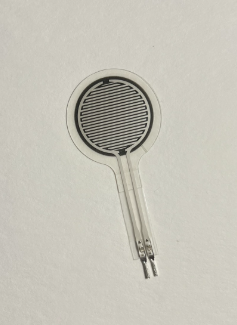
\includegraphics[,width=0.5\textwidth]{img/sensor.png}
        \caption{Sensor de fuerza MD30-60}
        \label{fig:Sensor de fuerza}
    \end{figure}